\documentclass[11pt,a4paper,ngerman]{article}
\usepackage[bottom=2.5cm,top=2.5cm]{geometry} 
\usepackage{babel}
\usepackage[utf8]{inputenc} 
\usepackage[T1]{fontenc} 
\usepackage{ae} 
\usepackage{amssymb} 
\usepackage{amsmath}
\usepackage{amsthm} 
\usepackage{graphicx}
\usepackage{fancyhdr}
\usepackage{fancyref}
\usepackage{listings}
\usepackage{xcolor}
\usepackage{paralist}

\usepackage[pdftex, bookmarks=false, pdfstartview={FitH}, linkbordercolor=white]{hyperref}
\usepackage{fancyhdr}
\pagestyle{fancy}
\fancyhead[C]{Computational Geometry}
\fancyhead[L]{Exercise sheet 9}
\fancyhead[R]{SoSe 2013}
\fancyfoot{}
\fancyfoot[L]{}
\fancyfoot[C]{\thepage \hspace{1px} of \pageref{LastPage}}
\renewcommand{\footrulewidth}{0.5pt}
\renewcommand{\headrulewidth}{0.5pt}
\setlength{\parindent}{0pt} 
\setlength{\headheight}{0pt}

\date{}
\title{Exercise sheet 9}
\author{Max Wisniewski, Alexander Steen}


%%
%% Enviroments for proofs and lemmas
%%
\newtheorem{lemma}{\bfseries Claim}

\begin{document}

\lstset{language=Pascal, basicstyle=\ttfamily\fontsize{10pt}{10pt}\selectfont\upshape, commentstyle=\rmfamily\slshape, keywordstyle=\rmfamily\bfseries, breaklines=true, frame=single, xleftmargin=3mm, xrightmargin=3mm, tabsize=2, mathescape=true}

\renewcommand{\figurename}{Figure}

\maketitle
\thispagestyle{fancy}

%%%%%%%%%%%%%%%%%%%%%%%%
%% Aufgabe 1 
%%%%%%%%%%%%%%%%%%%%%%%%
\subsection*{Problem 1}

Let $S$ be a set of sites in the plane, and let VD($S$) be the Voronoi diagram
for $S$.

\subsubsection*{(a)}

Let $s \in S$. Show that the Voronoi cell of $s$ is unbounded if and only if $s$
lies on the convex hull of $S$.\\

\textbf{Proof.}\\

$\Leftarrow$:\\

The voronoi cell VD($s$) is defined by the cut of all bisectors induced by $S$.
VS($s$) = $\underset{v \in S \setminus \{ s \}}{\bigcap} h(s,v)$.\\

Because VD($s$) is unbounded, we half a line $l$ through the cell VD($s$),
the will have all vertices of $S$ to its left and the
right is the unbounded part of VD($s$). This line can be moved, such that
$s$ is on this line. This can be done by moving the line by its normal in the
direction of $s$. If we hit another vertex $s'$ of $S$ then we rotate $l$ 
around $s'$ into the direction of $s$. It is obvious that the first part holds up the invariant,
that all $v \in S$ are on the left of the line.\\

In the second part we have to proove, that the first vertex, that will be hit
is the vertex $s$. Assume we hit another point $p \in S$ before we hit $s$,
then we have the situtation as in figure \ref{alge:ueb0:p1counter}

\begin{figure}[htbp]
    \centering
    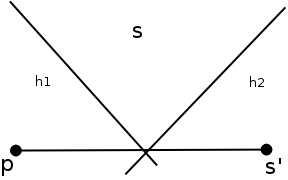
\includegraphics[width=0.6\textwidth]{media/p1counter}
    \caption{Rotate hits a third vertex first}
    \label{alge:ueb9:p1counter}
\end{figure}

We do not know, whether $h1, h2$ are part of the voronoi diagram, but
because VD($s$) = $\bigcap h(s,l)$ the right side of $l$ does no longer contain
the unbounded part of VD($s$).\\

Therefor we will hit the vertex $s$ first (or even in the translate step)
and $l$ satisfies the contdition, that alle points $v \in S$ are on the left.
Hence $s$ is a vertex of the convex hull.

$\Rightarrow$:\\

Let $s$ be a vertex in the convex hull. Then there exists a line $l$ through
$s$ such that any point $v \in S$ is on the left. Now any $h(s,v)$
will cut the line $l$ reflex from the inside (of the convex hull), 
because otherwise the point would have been to the right. Therefore
all bisectors have a degree greater then $90^\circ$ on the right side
of the convex hull. Because all lines have to start inside the convex hull
we can only try to bound VD($s$) with a triangle, but we already know, that
for any two angles we have a degree greater then $180^\circ$.
Hence we cannot bound VD($s$) on the right of $l$ and VD($s)$ is unbounded.

\mbox{}\hfill$\square$

\subsubsection*{(b)}

Conclude that any comparison-based algorithm for computing VD($S$) requires
$\Omega (n \log n)$ steps.

\textbf{Proof.}\\

As shown previously the computation of the convex hull requires $\Omega (n \log n)$ steps.\\

Assume the runningtime of voronoi-diagram is $T(n)$. Then we can use the following 
algorithm to compute the convex hull.\\

\begin{enumerate}[1.]
    \item Compute the voronoi diagram VD($S$).
    \item Perform a depth first search on the resulting Graph where $s$ are the vertices and
        an edge exists of two cells are neighbours, for the first unbounded cell.
    \item From one unbounded cell, there is an edge to the next and previous unounded cell. Fix
        on direction and iterate, until the first one is reached.
\end{enumerate}

This approach works, because two successiv vertices in the convex hull share an edge in the voronoi diagram,
because this edge is unbounded. If there would be something inbetween that cuts this unbounded edge it would
have to be unbounded itself and therefor both sites are not succesiv in the convex hull.\\

The running time is
    $$ T'(n) = T(n) + O(n) + O() = T(n) + O(n)$$
and because we know that $T'(n) \in \Omega (n \log n)$ the
only possibility is, that $T(n) \in \Omega (n \log n)$ because
$O(n)$ can not tribute to this bound.

\mbox{}\hfill $\square$

\subsection*{Problem 2}

\subsubsection*{(a)}

Give an example where the bisector $B(s,l)$ between some site and the sweepline
contributes more then one arc to the wavefront. Can you give an example where
it contributes a linear number of arcs?\\

\textbf{Solution.}\\

\begin{figure}[bt]
    \centering
    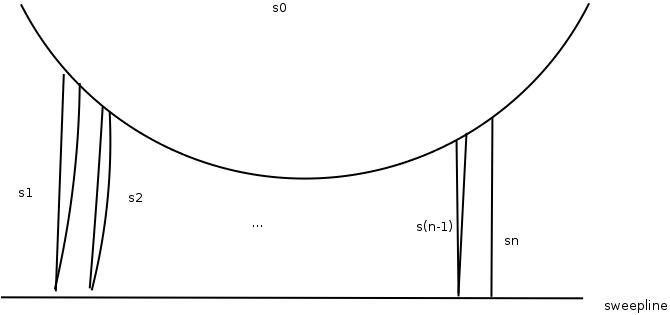
\includegraphics[width=0.8\textwidth]{media/p2ex1}
    \caption{Sweepline with a linear number of arc fragments}
    \label{alge:ueb9:linarcs}
\end{figure}

As we can see in figure \ref{alge:ueb9:linarcs} if we have a single site
to the top and many sites at nearly the same $y$ coordinate far enough apart
that after the last is considered from the sweepline no arcs of these will met,
then the arc of $s_0$ will be cut by each of the $n$ remaining sites and
the wace of $s_0$ will be cut into $n+1$ arcs.

\subsubsection*{(b)}

Give an example of six sites such that Forutne's sweep encounters all site
events before any circle event. The sites should be in general position.\\

\textbf{Solution.}\\

If all points lie extremly close and nearly on a circle with the middle point far enough away in $y$ direction.\\
Assume all lie on a circle, then we shake the points a bit, such that the middlepoints are not the same
(we need to do this, because the general position assumption for the algorithm was, that not more
then three points lie on a circle).
But as constructed the circle events lie far below all points, because the circle event is the middlepoint of the circle.

\vspace{5cm}

\subsection*{Problem 3}

Let $S$ be a set of $n$ sites in the plane.

\subsubsection*{(a)}

Give an algorithm that in $O(n \log n)$ time finds for each $s \in S$ the site in
$S \setminus \{s \}$ that is closest to $s$. Prove that your algorithm is correct.\\

\textbf{Solution.}\\

The algorithm does the following.
\begin{enumerate}
    \item Compute the Voronoi diagram.
    \item Iterate over the graph with sites as vertices and edges, if two cells are connected by an edge.
          And do for every site the following
        \begin{enumerate}[a.]
            \item For every adjacent site, compute the distant to the site and take the smallest one.
        \end{enumerate}
\end{enumerate}

This algorithm runs in $O(n \log n)$, because we can copmute the Voronoi diagram in $O(n \log n)$.
The loop that checks all neighbours for the distant will compute the distants for every edge
exactly twice (one time from each site). As we have prooven in lecture there are $O(n)$ edges
and therefor the running time is
$$ T(n) = O(n \log n) + O(n) = O(n \log n). $$

\begin{lemma} \label{alge:ueb9:t3:cor} The algorithm is correct.
\end{lemma}

\textbf{Proof \ref{alge:ueb9:t3:cor}.}\\
To proove correctness, we have to show, that the closest site to a given site $S$ has to be a neighbour cell
in VD($S$).\\

We have shown in the lecture, that a point is in VD($S$), if it is the center of a circle with two points
of $S$ on the boundary and no points in its interior.

Now let $s$ be some site and $s' \in S \setminus \{ s \}$ the closest point. Now the circle centered at the point
in the middel of $m \overline{ss'}$ $C = B_{\frac{1}{2}\text{dist}(s,s')}(m)$ cannot contain any other point in $S$,
because the distance from $s$ to any point in $C$ is smaller then dist($s,s'$).\\

Because we know there are at most 3 points of $S$ on a circle, we can move this circle to at least on direction where
still $s,s'$ are on its boundary and no point is in its interior, by moving it away from the third point if one exists
or simply on the normal of the line $\overline{ss'}$ at $m$.\\
Therefor the voronoi cell VD($s$) shares an edge with the voronoi diagram VD($s'$) which is closest. Therefor
the closest site will be checked in the loop and because the smallest one will be taken, $s'$ is picked for $s$.
\mbox{} \hfill $\square$

\subsubsection*{(b)}

Give an algorithm that in $O(n \log n)$ time finds the largest circle $C$ such that the center of $C$ lies inside the convex hull of $S$ and such that $C$ does not contain any sites in its interior. Prove that your algorithm is correct.\\

\textbf{Solution.}\\

We assume that no three points lie on a line.

The algorithm is the following one.
\begin{enumerate}[1.]
    \item Compute the voronoi diagram VD($S$).
    \item Consider the graph $G$ where the vertices are the vertices of VD($S$) (three cells meet)
        and the edges are edges of VD($S)$ (exactly two cells meet). Iterate over the
        vertices of $G$.
        \begin{enumerate}[a.]
            \item Compute the distants to one of the meeting cells in this point. If the
                distants if greater then the previously greatest circle, take this as the newest
                greatest circle.
        \end{enumerate}
\end{enumerate}

\begin{lemma} \label{alge:ueb9:t4:cor}
    The algorithm is correct and runs in time $O(n \log n)$.
\end{lemma}

\textbf{Proof \ref{alge:ueb9:t4:cor}.}\\

The first step takes $O(n \log n)$ to compute. As we have shown in lecture there are $O(n)$ vertices,
such that the second loop takes $O(n)$ time total, if we stored the sites for every vertex in the construction.\\

Therefor the runningtime is
$$ T(n) = O(n \log n) + O(n) = O(n \log n).$$

For the correctness we first have to see, that the possible circles are the vertices of the voronoi diagram.\\
Consider a circle $C$ centered in the propper interior of a cell VD($s$) with middle point $m$. The circle has the size $\pi \text{dist}(m,s)$.
This circle is empty, because $m$ is in VD($s$) and therefor there is no other point in $S$ with a smaller distance to $m$.\\
If we move $m$ to the boundary of VD($s$) in direction $\overrightarrow{sm}$, the radius of the ball will increase. The circle will stay empty
as long as we are in the interior of VD($s$). Therefor the biggest circle has to be centered on the boundary of a cell.\\

Next we have to show, that only vertices of VD($S$) are possible choices. Let $B_r(m)$ be a circle centered in the proper interior of an 
edge of VD($S$). Then there are two sites $s,s'$ with distance $r$ to $m$. Let $d$ be the middle point of $\overline{s,s'}$
the radius increases, if we move the ball in direction $\overrightarrow{dm}$ (some normal if $m = d$) by triangle inequality.\\

It is always possible to move the ball by at least an $\varepsilon > 0$, because there is no third site on the boundary.\\

We have two things remaining to show. First all vertices lie within the convex hull and that the $C$ can only be centered at a vertex.\\
The first thing holds, because a voronoi vertex has three sites such that the maximal empty circles cut all in the vertex. Therefor
the vertex lies in the interior of the triangle of these three sites.\\
By the incremental construction of the convex hull we know, that if we add a point, the previous interior remains interiour, such that
after adding all sides the vertex is still in the interior of the convex hull.\\

We know that we can move the circes along the edges and increase their radi. Therefor we hit a vertex or we run into an unbounded edge.\\
As shown in problem 1, an unbounded edge has two vertices $s,s'$ of the convex hull as meeting cells. There the middle point of the line $\overline{s,s'}$
lies on the convex hull. The problem allows only points inside the convex hull. At this point we can only move the ball towards the inside.
And as we have shown this increases the radius. Therefor we do not have to consider the unbounded edges, because they maximize inside the convex hull
at a vertex.\\

Because of general position assumptions there exists vertices in the voronoi diagram.\\

Last we checked all vertices of the voronoi diagram and took the greatest circle. Hence the algorithm is correct.

\mbox{}\hfill $\square$

\label{LastPage}


\end{document}
